\section{Evaluation}
\label{sec:Eval}
\subsection{Profiling and Performance Considerations}
We profile the client execution on a large set of queries. Our profiling is mainly offline to assess the implementations' resource usage. The main profiling tool that we use is the Linux \texttt{time} utility with a custom format string (as shown below):
\begin{lstlisting}
#!/bin/bash
/usr/bin/time -o "/tmp/profiling" --append -f "%e real,\t%U user,
\t%S sys,\t%P CPU, \t%Mk max mem,\t%F major pagefaults,
\t%R minor pagefaults" pypy3 client.py);
\end{lstlisting}

The syscall used in \texttt{time} command is wait4. In linux, the parent process can query whether the child process terminates through the wait4() system call \cite{wait4}. wait4() function can obtain not only the status information of the sub-process, but also the resource utilization information of the sub-process, which is obtained through the parameter usage. 

\subsubsection{Runtime Systems Benchmarks}
In this project we worked with \texttt{PyPy} and \texttt{CPython} runtime systems which briefly described below.
\begin{center}
\begin{table}[h]
 \caption{Comparison between PyPy and CPython}
\begin{tabular}{ | l | p{5cm} |p{5cm} |} 
 \hline
  & PyPy \cite{pypy}  & CPython \cite{cpython} \\ 
  \hline
  Runtime System & just-in-time compiler & Mixed mode (interpreter with profile guided optimization)  \\ 
  \hline
 Garbage Collection Algorithm & Incminimark (incremental with generational moving collector) & Reference Counting \\ 
 \hline
\end{tabular}
\end{table}
\end{center}

\subsubsection{Profiling - Execution Time}
Here, we are comparing the execution time of the program within different runtime systems. 
\hspace*{-0.8in}
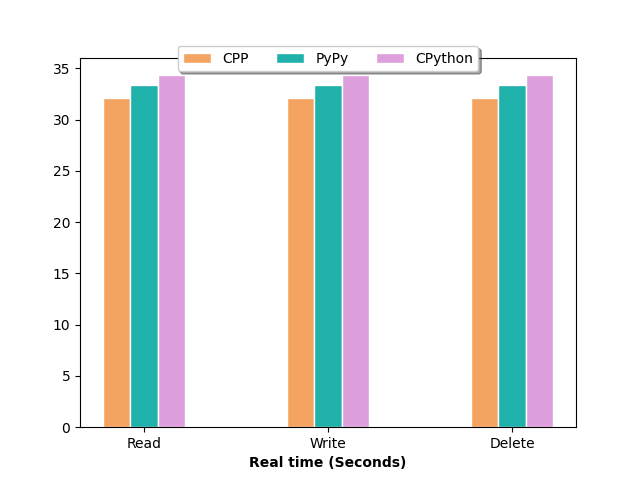
\includegraphics[width=9.5cm, height=8cm]{sections/Figures/real_time.png}
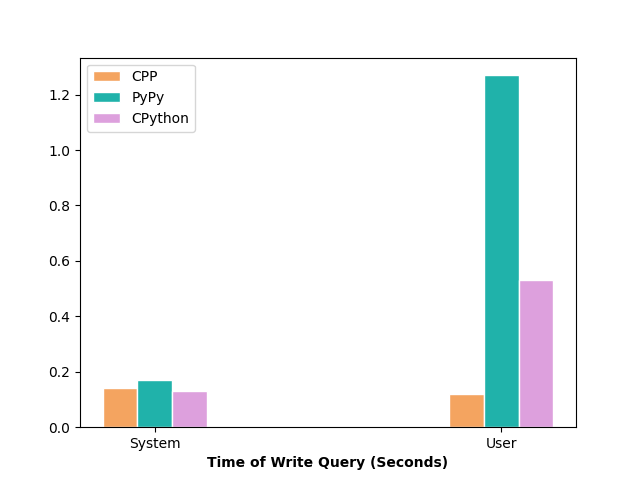
\includegraphics[width=9.5cm, height=8cm]{sections/Figures/time_user_sys.png}


\texttt{real time} refers to actual elapsed time - time from start to finish of the call. \texttt{User} is the amount of CPU time spent in user-mode code within the process. This is only actual CPU time used in executing the process. Similarly, \texttt{Sys} is the amount of CPU time spent in the kernel within the process. As you can see the figures above, our program spends most of the time in user mode. \texttt{PyPy} is the slowest among the CPython and C++ executable mainly due to the time PyPy runtime spent for compilation of the codes that runs once in our program. The left chart, shows our program has a lot of network connection and while CPU is not involved, the process is waiting for network responses.

\subsubsection{Profiling - CPU Usage}
As mentioned above, our program does not have heavy computation and CPU is not too involved. You can see the CPU usage of the program in the chart below. C++ CPU usage is 0\% but PyPy used CPU up to 3\%.

\begin{center}
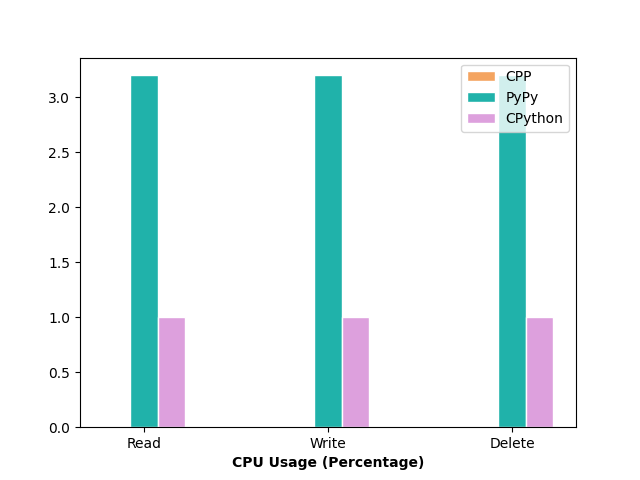
\includegraphics[width=9.5cm, height=8cm]{sections/Figures/cpu.png}
\end{center}

\subsubsection{Profiling - Memory Usage}
Based on the memory usage result, PyPy used more memory than the others and it refers to the memory PyPy takes for compilation purposes. In the right chart, the number or minor page faults are shown. Since, CPython uses reference counting GC it reserves the locality of references in memory and causes less page faults. 

\hspace*{-0.8in}
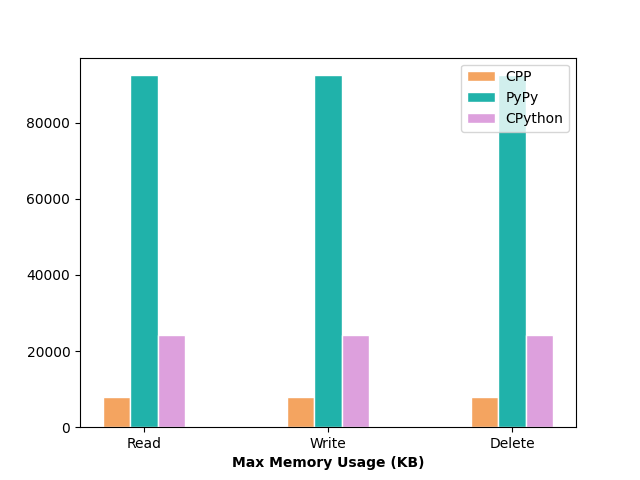
\includegraphics[width=9.5cm, height=8cm]{sections/Figures/max_memory.png}
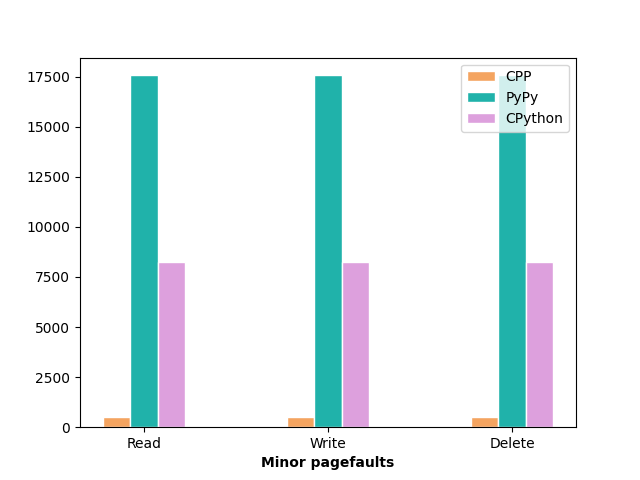
\includegraphics[width=9.5cm, height=8cm]{sections/Figures/minor_pagefault.png}
